\section{Conception}
Nous avons choisi d'utiliser un module externe au téléphone mobile pour la mesure par ultrasons. Ce module est connecté à un Arduino munis d'un bloc de communication Bluetooth.\\
Nous avons donc une application sur smartphone qui communique par Bluetooth standard avec un Arduino équipé d'un module de télémétrie.
\begin{figure}[H]
	\begin{center}
		\includegraphics[width=10cm]{img/schemaBloc.png}
		\caption{Illustration de la communication}
		\label{schemabloc}
	\end{center}
\end{figure}
Ce projet à donc été séparé en deux parties distinctes, à savoir la programmation sur Android et celle sur Arduino.\\
Nous avons réaliser une première représentation de ce que nous voulions pour le projet.
\begin{figure}[H]
	\begin{center}
		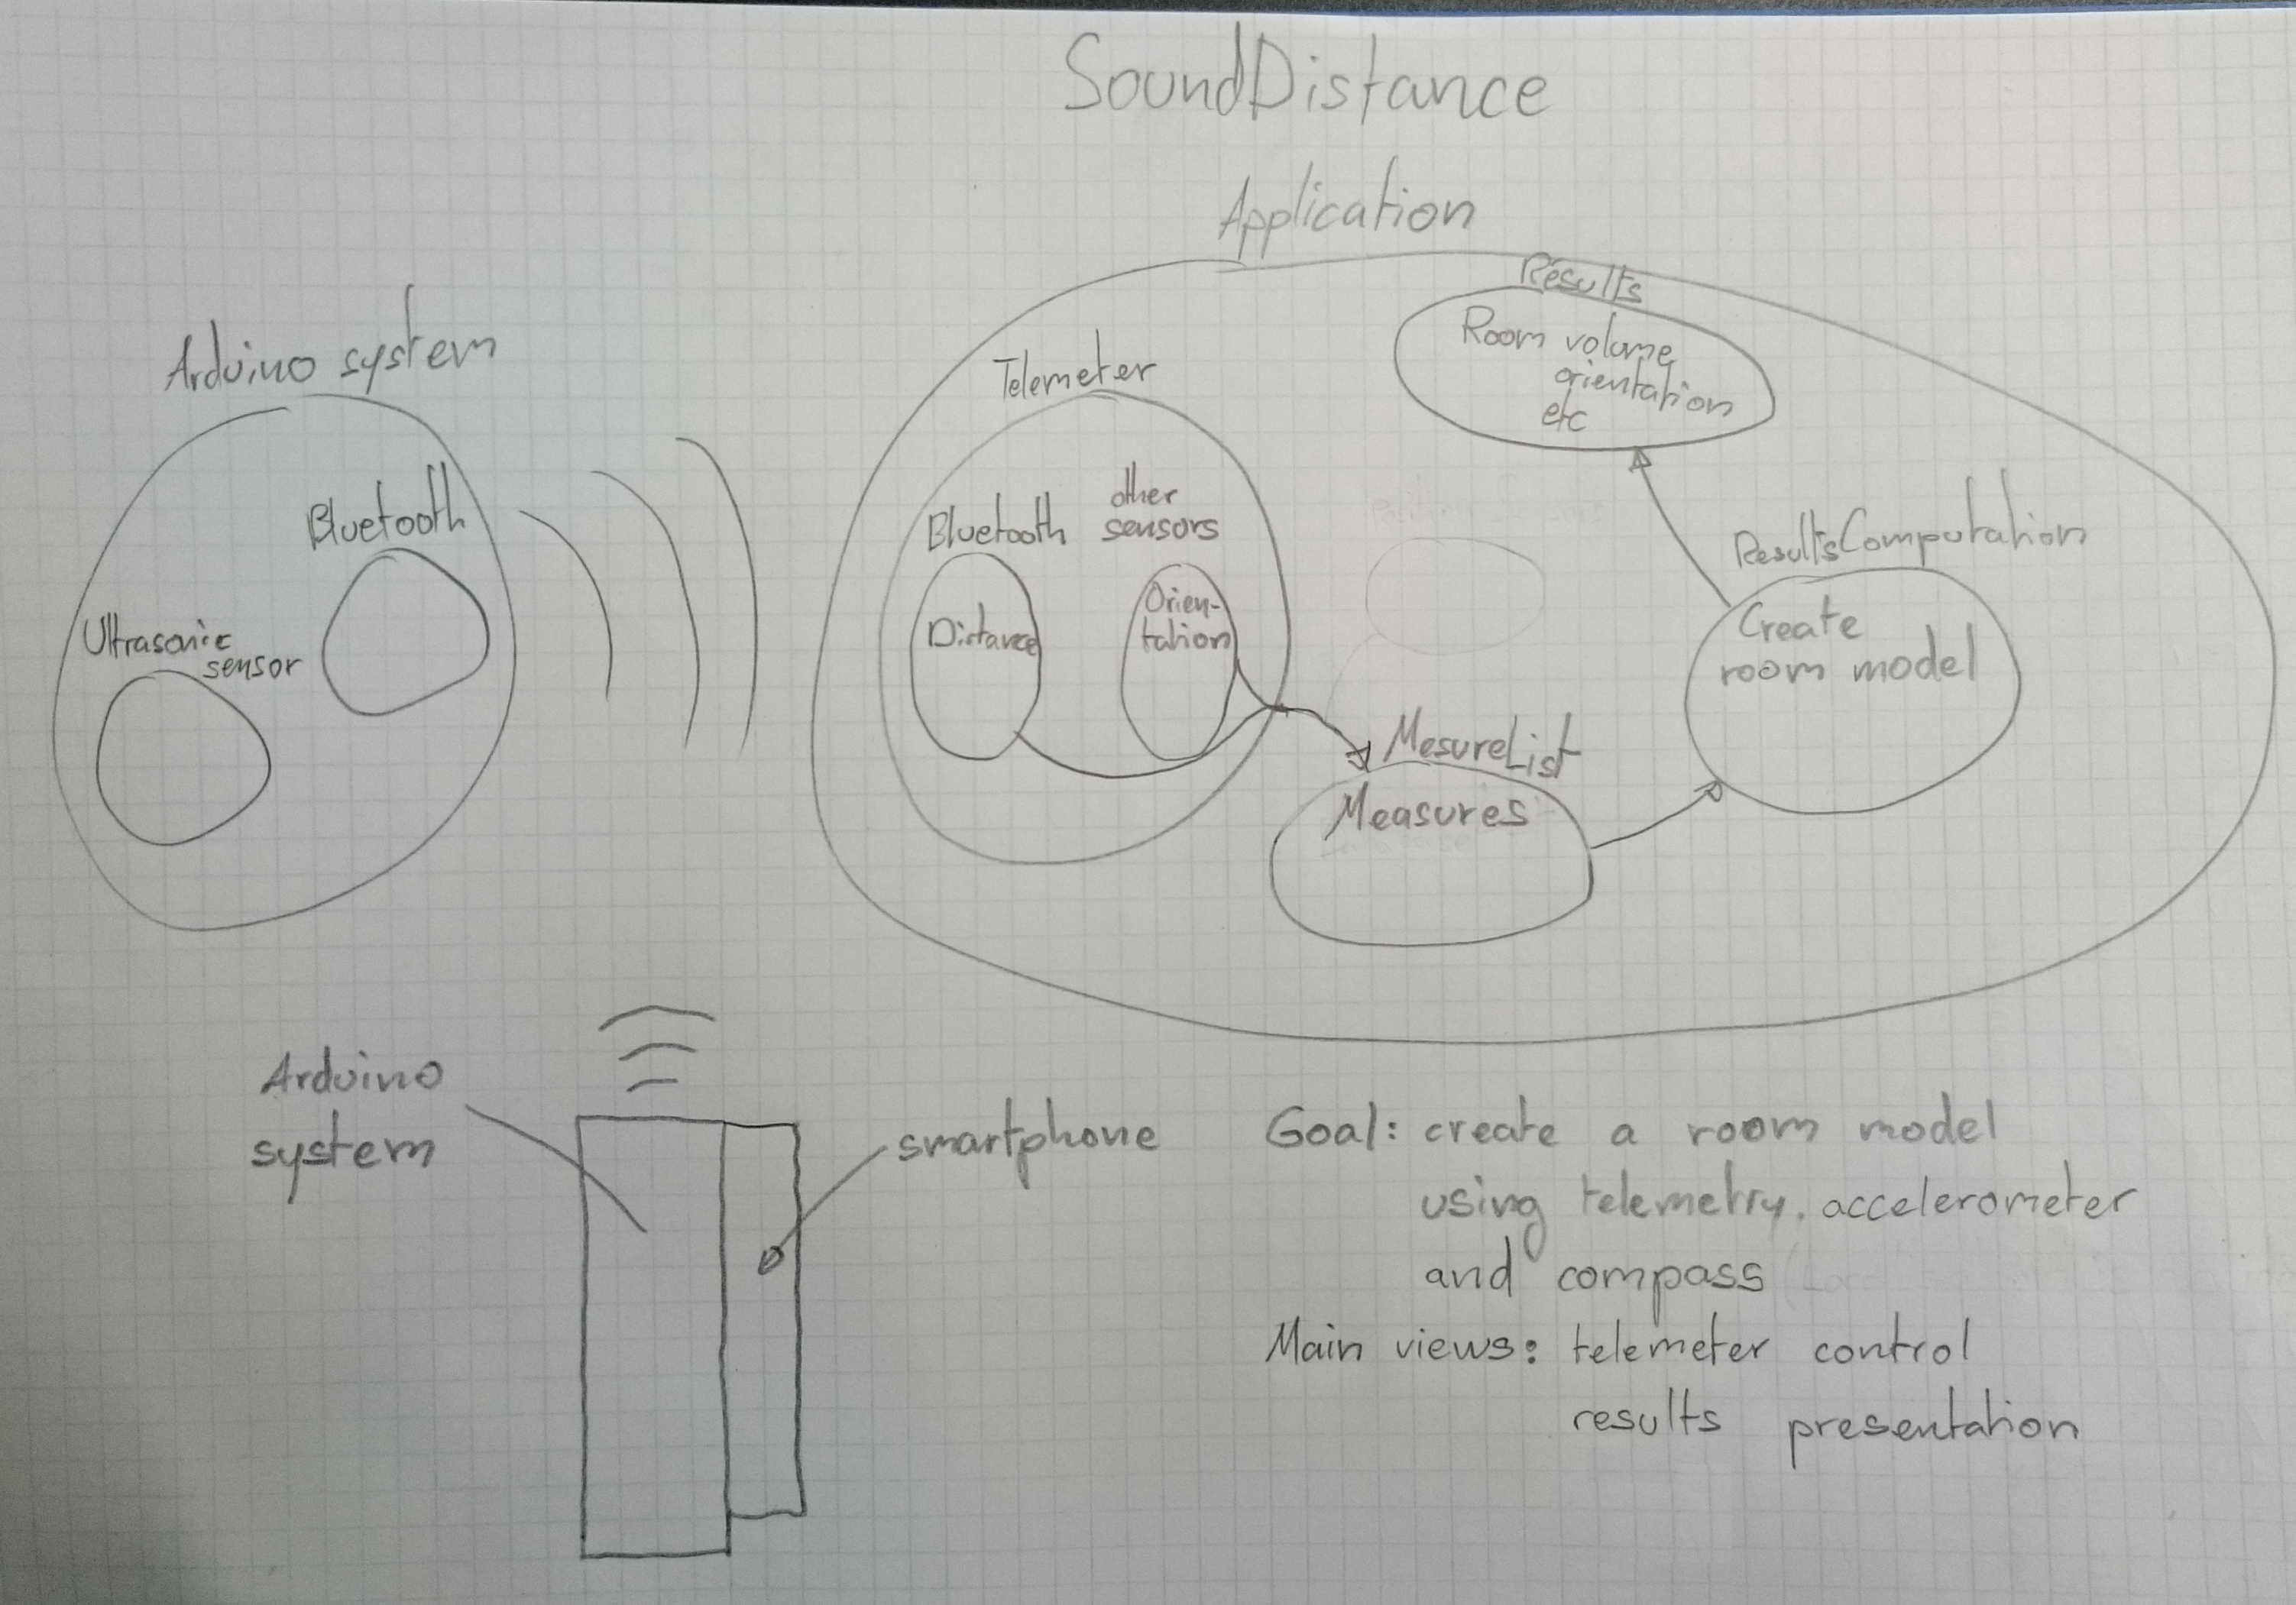
\includegraphics[width=11.8cm]{img/concep0.png}
		\caption{Définition de la structure du projet}
		\label{conception0}
	\end{center}
\end{figure}
La partie "Arduino System" a été développé conformément au dessin avec les deux parties bluetooth et ultrasonic sensor.\\
Les différentes parties définies pour l'application Android ont été utilisées pour le développement. Nous avions décidé, dans un premier temps, d'utiliser divers capteurs comme l'accéléromètre et le compas pour avoir des informations sur l'orientation de la mesure, mais nous avons rejeté cette idée d'un commun accord avec notre professeur, car elle n'apportais pas grand chose aux mesures et compliquait l'interprétation des résultats.\\
Nous avions également dans l'idée de créer un boîtier pour l'Arduino avec le capteur à ultrason. Nous voulions faire en sorte que le smartphone puisse être intégré au boîtier. \\
Après réflexion, nous avons jugé plus judicieux de séparé l'Arduino du smartphone, car cela n'aurait pas été pratique pour prendre les mesures.\\\\
Sur cette base, nous avons été en mesure de respécifier les buts du projet. Nous allons donc réaliser une application Android permettant la mesure de distance par ultrason à l'aide d'un capteur externe sur Arduino. L'application servira uniquement à mesurer des espaces fermés comme des pièces de maison. On aura le choix entre trois types de mesure: une distance, une aire ou un volume.\\
Sur la base de ce cahier des charges, nous avons établis sur papier la représentation des différentes vues de l'application avec leur contenu et les informations passées entre elles. Nous nous sommes ensuite séparé le travail à réaliser.
\begin{figure}[H]
	\begin{center}
		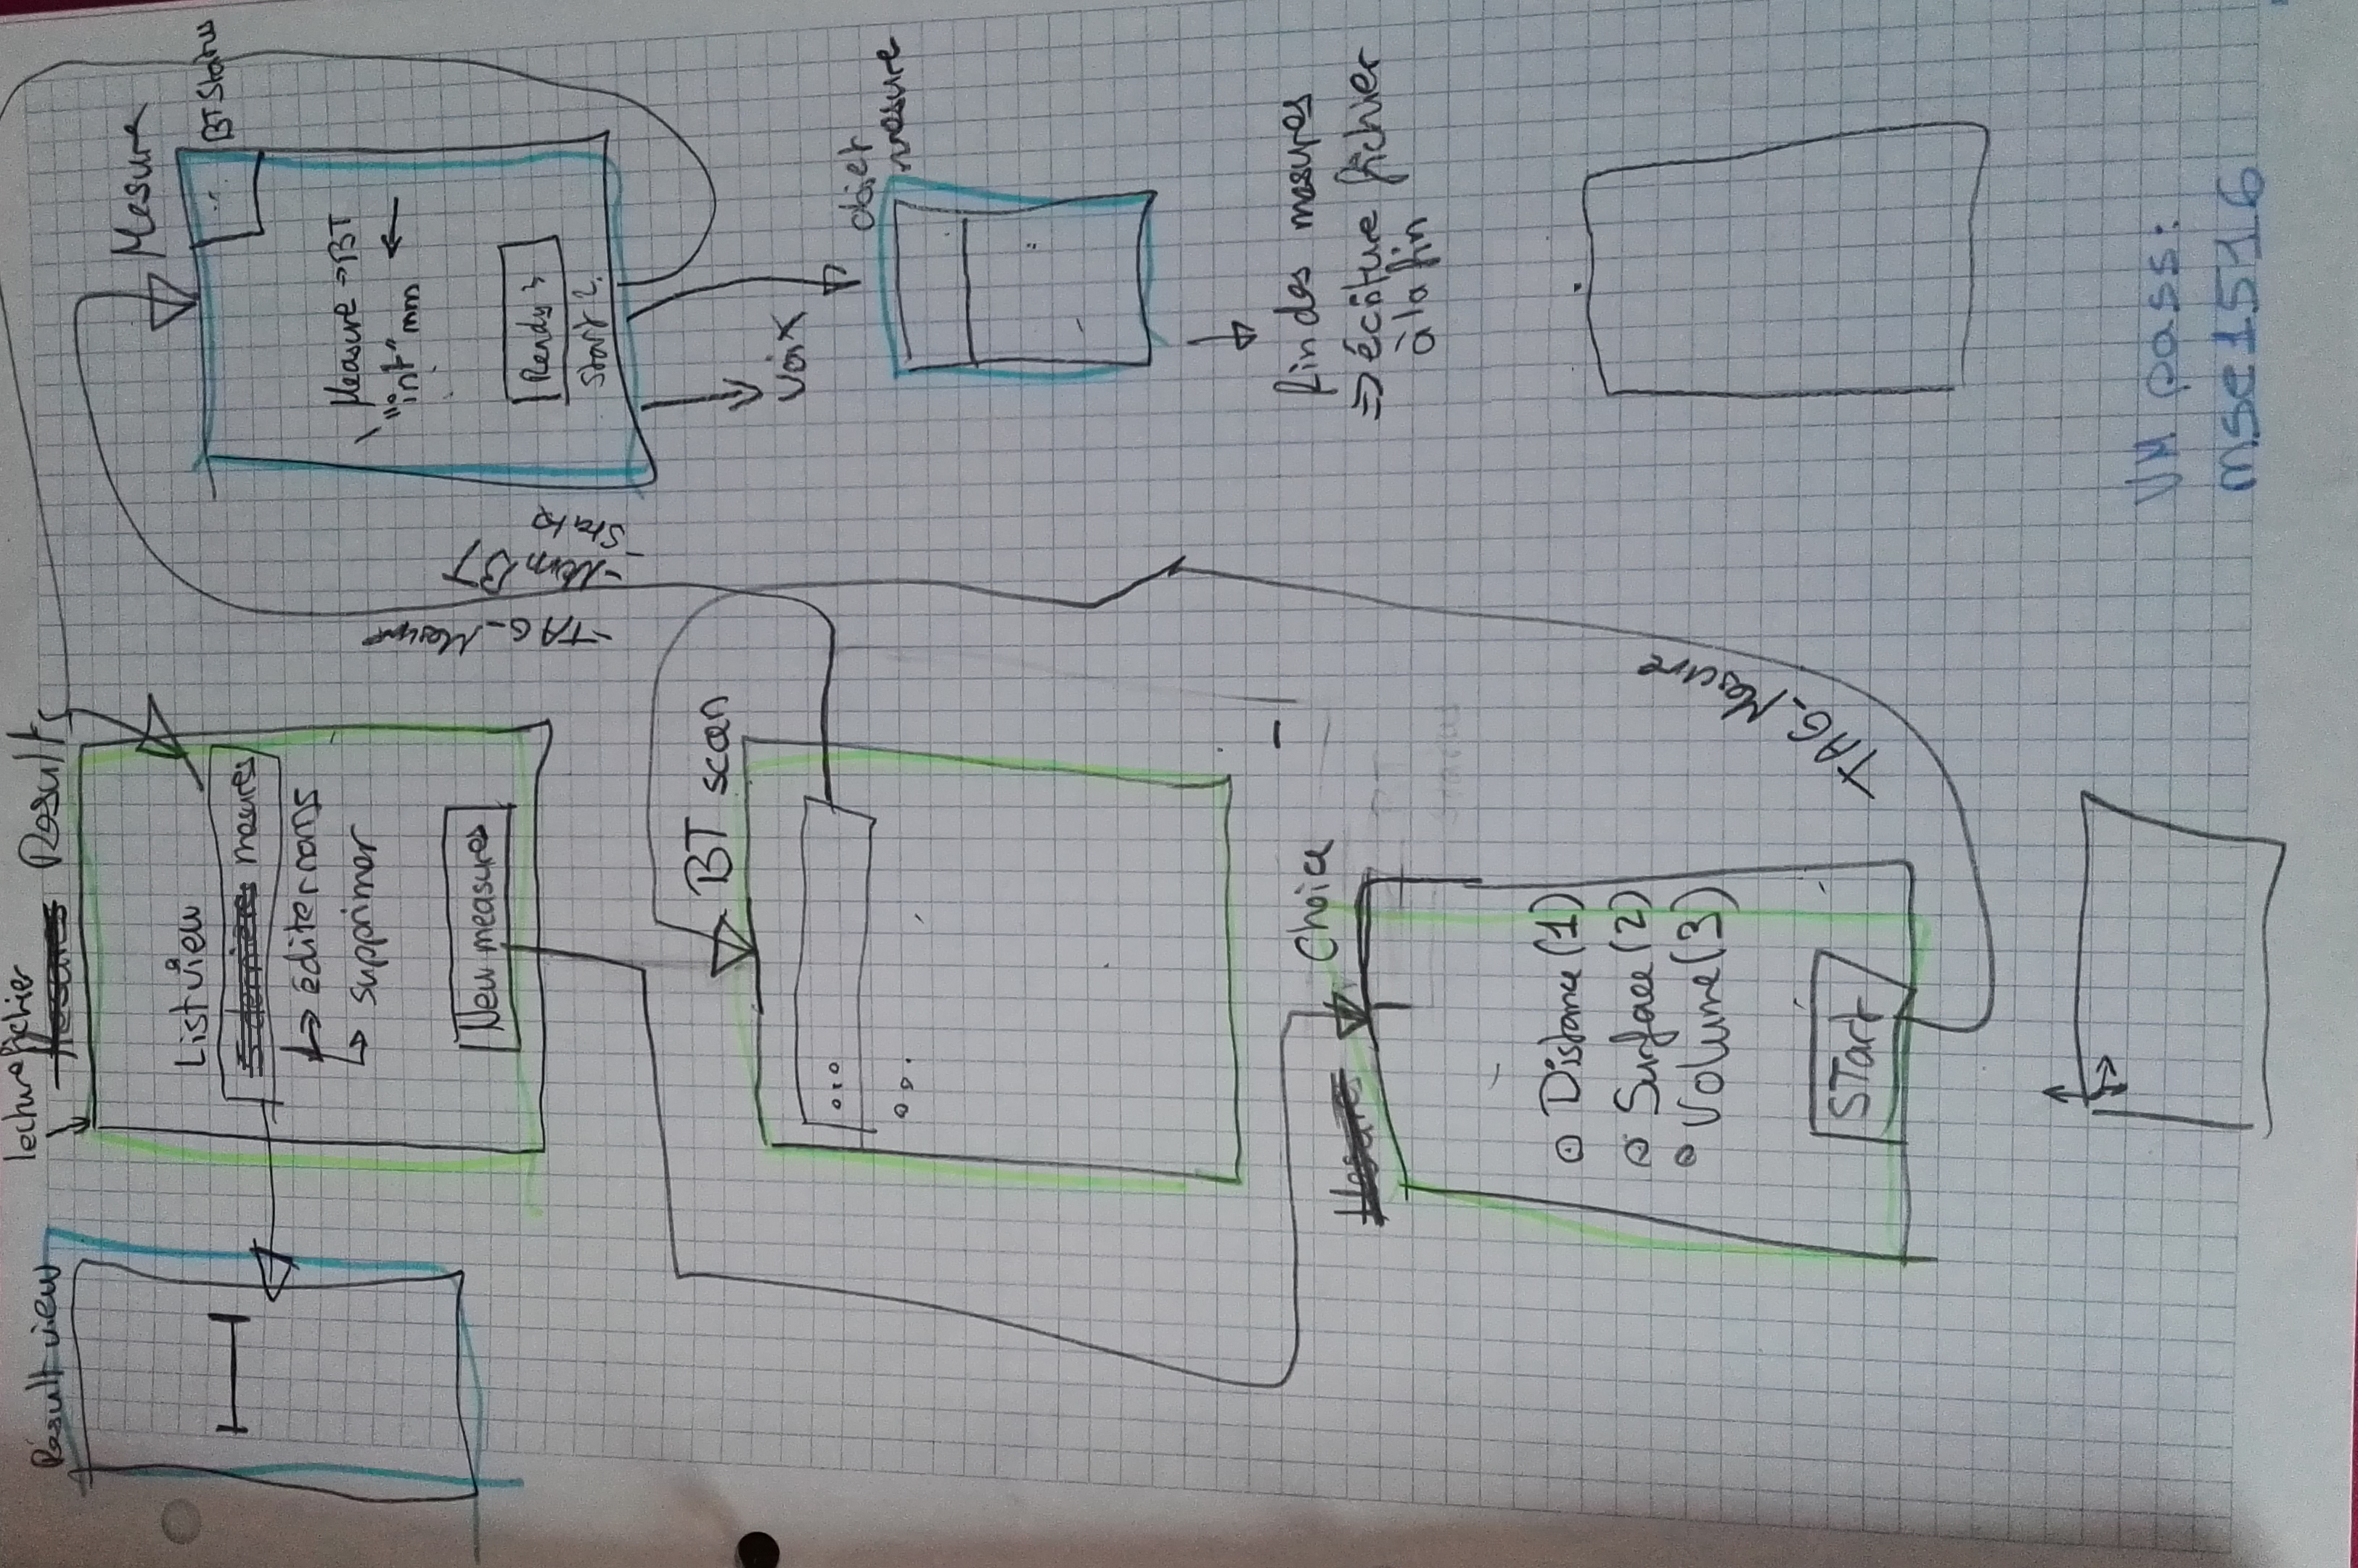
\includegraphics[width=17cm]{img/concep1.png}
		\caption{Définition des différentes vues}
		\label{conception1}
	\end{center}
\end{figure}
